\documentclass[11pt,class=report,crop=false]{standalone}
\usepackage[screen]{../python}

\begin{document}


%====================================================================
\chapitre{Python : numpy et matplotlib avec deux variables}
%====================================================================

\insertvideo{jZjAeBVj9tw}{partie 4.1. Numpy}

\insertvideo{contVfU2b-w}{partie 4.2. Matplotlib}

\begin{center}
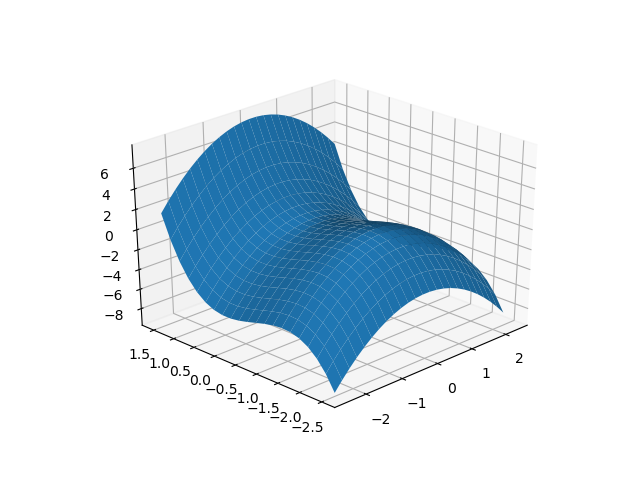
\includegraphics[scale=\myscale,scale=0.6]{figures/pythonxy-intro1}
\end{center}

\objectifs{Le but de ce chapitre est d'approfondir notre connaissance de \numpy{} et \matplotlib{} en passant à la dimension $2$. Nous allons introduire les tableaux à double entrée qui sont comme des matrices et visualiser les fonctions de deux variables.}

\medskip

\objectifs{Voici le graphe de la fonction $f(x,y) = y^3 + 2y^2 - x^2$ (ci-dessus et ci-dessous à gauche, dessinés sous deux points de vue différents) ainsi que ses lignes de niveau dans le plan (ci-dessous à droite).}


\begin{center}
  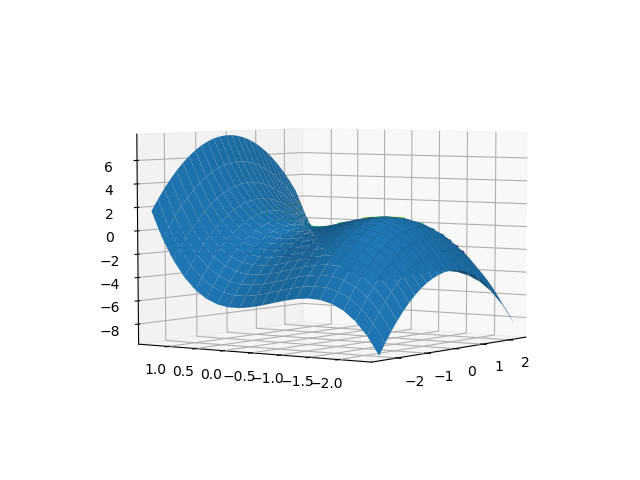
\includegraphics[scale=\myscale,scale=0.4]{figures/pythonxy-intro2}
  \quad
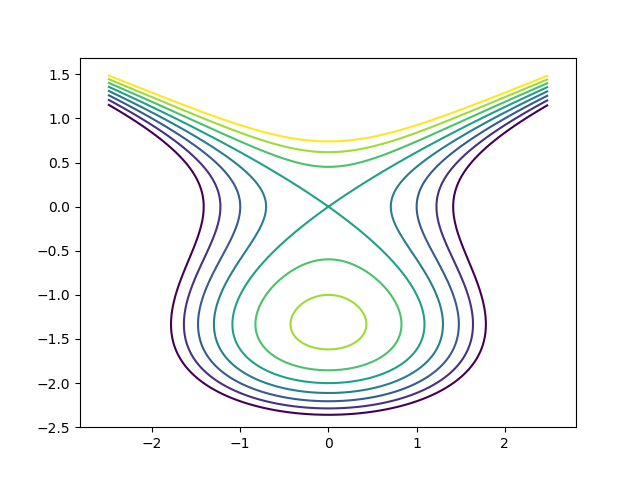
\includegraphics[scale=\myscale,scale=0.4]{figures/pythonxy-intro3}
\end{center}

%%%%%%%%%%%%%%%%%%%%%%%%%%%%%%%%%%%%%%%%%%%%%%%%%%%%%%%%%%%%%%%%%%%%%
\section{Numpy (deux dimensions)}

Nous avons vu comment définir un vecteur (un tableau à une dimension), comme par exemple \ci{[1 2 3 4]}. Nous allons maintenant étudier les tableaux à deux dimensions.

%--------------------------------------------------------------------
\subsection{Tableau}

Un tableau à deux dimensions est comme une matrice (ou un tableau à double entrée).

\begin{itemize}
  \item \textbf{Définition.} Un tableau se définit comme une suite de lignes
\mycenterline{\ci{A = np.array([[1, 2, 3], [4, 5, 6]])}}
(en ayant au préalable importé et renommé le module \numpy{} en \ci{np}) et s'affiche ainsi :
  \begin{center}
  \begin{minipage}{0.15\textwidth}
\begin{lstlisting}
[[1 2 3]
 [4 5 6]]
\end{lstlisting}
  \end{minipage}
  \end{center}
  
 C'est un tableau à deux lignes et trois colonnes qui correspond à la matrice :
 $$\begin{pmatrix}1&2&3\\4&5&6\end{pmatrix}.$$

  \item \textbf{Taille.}\index{numpy@\numpy!shape@\ci{shape()}}  On récupère la taille du tableau par la fonction \ci{shape()}.  Par exemple \ci{np.shape(A)} renvoie ici $(2,3)$, pour $2$ lignes et $3$ colonnes.
  
  \item \textbf{Parcourir les éléments.} On accède aux éléments par des instructions du type \ci{A[i,j]} où $i$ est le numéro de ligne et $j$ celui de la colonne. Voici le code pour afficher les éléments un par un.
  
  \begin{minipage}{0.59\textwidth}
  \myfigure{0.6}{
    \tikzinput{fig-tableau}
  } 
  \end{minipage}
  \begin{minipage}{0.4\textwidth}
\begin{lstlisting}
p, n = np.shape(A)
for i in range(p):
	for j in range(n):
		print(A[i,j])
\end{lstlisting}
  \end{minipage}
  
  \item \textbf{Fonctions.} Les fonctions s'appliquent élément par élément. Par exemple \ci{np.sqrt(A)} renvoie un tableau ayant la même forme, chaque élément étant la racine carrée de l'élément initial.
  \begin{center}
  \begin{minipage}{0.5\textwidth}
\begin{lstlisting}
[[1.         1.41421356 1.73205081]
 [2.         2.23606798 2.44948974]]
\end{lstlisting}
  \end{minipage}
  \end{center}  
  
  \item \textbf{Définition (suite).} \ci{np.zeros((p,n))} renvoie un tableau de $p$ lignes et $n$ colonnes rempli de $0$. La fonction \ci{np.ones()} fonctionne sur le même principe.

\end{itemize} 

%--------------------------------------------------------------------
\subsection{Conversion tableau-vecteur}

Il est facile et souvent utile de passer d'un tableau à un vecteur et réciproquement.

\begin{itemize}
  \item \textbf{Tableau vers vecteur.} On obtient tous les éléments d'un tableau regroupés dans un vecteur par la commande d’aplatissement \ci{flatten()}.
  Par exemple si 
  \mycenterline{\ci{A = np.array([[1, 2, 3], [4, 5, 6]])}} 
  alors la commande \ci{X = A.flatten()}\index{numpy@\numpy!flatten@\ci{flatten()}} renvoie le vecteur $X$ :
\mycenterline{\ci{[1 2 3 4 5 6]}}

\item \textbf{Vecteur vers tableau.} L'opération inverse se fait avec la fonction \ci{reshape()}\index{numpy@\numpy!reshape@\ci{reshape()}} qui prend en entrée la nouvelle taille désirée.
Par exemple : \ci{X.reshape((2,3))} redonne exactement \ci{A}.
Par contre \ci{X.reshape((3,2))} renvoie un tableau à $3$ lignes et $2$ colonnes :
  \begin{center}
  \begin{minipage}{0.2\textwidth}
\begin{lstlisting}
[[1 2]
 [3 4]
 [5 6]]
\end{lstlisting}
  \end{minipage}
  \end{center}  
  
\end{itemize}


%--------------------------------------------------------------------
\subsection{Fonctions de deux variables}


\begin{itemize}
  \item \textbf{\'Evaluation sur des vecteurs.} 
Supposons que nous ayons défini une fonction \Python{} de deux variables \ci{f(x,y)}.
Si \ci{VX} et \ci{VY} sont deux vecteurs de même taille, alors
\ci{f(VX,VY)} renvoie un vecteur composé des $f(x_i,y_i)$ pour $x_i$ dans \ci{VX} et $y_i$ dans \ci{VY}.
Par exemple, si \ci{VX} vaut \ci{[1 2 3 4]} et \ci{VY} vaut \ci{[5 6 7 8]}
alors \ci{f(VX,VY)} est le vecteur de longueur $4$ composé de $f(1,5)$,
$f(2,6)$, $f(3,7)$, $f(4,8)$. Mais ceci n'est pas suffisant pour tracer des fonctions de deux variables. 
  \item \textbf{Grille.} 
Pour dessiner le graphe d'une fonction $f(x,y)$, il faut calculer des valeurs $z=f(x,y)$ pour des $(x,y)$ parcourant une grille. Voici comment définir simplement une grille à l'aide \ci{meshgrid()}.\index{numpy@\numpy!meshgrid@\ci{meshgrid()}}

\begin{lstlisting}
n = 5
VX = np.linspace(0, 2, n)
VY = np.linspace(0, 2, n)
X,Y = np.meshgrid(VX, VY)

def f(x,y):
	return x**2 + y**2

Z = f(X,Y)
\end{lstlisting}

  \item \textbf{Explications.}
  \begin{itemize}
    \item \ci{VX} est un découpage de l'axe des $x$ en $n$ valeurs.
    \item \ci{VY} est la même chose pour l'axe des $y$.    
    \item \ci{X} et \ci{Y} renvoyés par \ci{meshgrid()} forment la grille. Ce sont des tableaux $n\times n$. Le premier représente les abscisses des points de la grille, le second les ordonnées. (Ce n'est pas très naturel mais c'est comme ça !)
     
     \myfigure{0.6}{
        \tikzinput{fig-grille}
      } 
    
\bigskip

\begin{center}
\begin{minipage}{0.45\textwidth}
Tableau \ci{X}
\begin{center}
\begin{lstlisting}
[[0.  0.5 1.  1.5 2. ]
 [0.  0.5 1.  1.5 2. ]
 [0.  0.5 1.  1.5 2. ]
 [0.  0.5 1.  1.5 2. ]
 [0.  0.5 1.  1.5 2. ]]
\end{lstlisting}
\end{center}
\end{minipage}
\begin{minipage}{0.45\textwidth}
Tableau \ci{Y}
\begin{center}
\begin{lstlisting}
[[0.  0.  0.  0.  0. ]
 [0.5 0.5 0.5 0.5 0.5]
 [1.  1.  1.  1.  1. ]
 [1.5 1.5 1.5 1.5 1.5]
 [2.  2.  2.  2.  2. ]]   
\end{lstlisting}
\end{center}
\end{minipage} 
\end{center}

    \item Enfin \ci{Z = f(X,Y)} calcule les valeurs $z = f(x,y)$ pour tous les éléments de $(x,y)$ de la grille et renvoie un tableau des valeurs.  
\begin{center}
\begin{minipage}{0.45\textwidth}
Tableau \ci{Z}
\begin{center}
\begin{lstlisting}
[[0.   0.25 1.   2.25 4.  ]
 [0.25 0.5  1.25 2.5  4.25]
 [1.   1.25 2.   3.25 5.  ]
 [2.25 2.5  3.25 4.5  6.25]
 [4.   4.25 5.   6.25 8.  ]]
\end{lstlisting}
\end{center}
\end{minipage}  
\end{center}    
  
    
  \end{itemize}
  
  \item \textbf{Points.} Ainsi $X,Y,Z$ forment une liste des $n^2$ points de l'espace dont on donne d'abord l'abscisse (dans $X$), puis l'ordonnée (dans $Y$), puis la hauteur (dans $Z$).
  Si on augmente la valeur de $n$, on commence à voir apparaître la surface d'équation $z=f(x,y)$. Ci-dessous le cas $n=5$ à gauche et $n=20$ à droite.
  
  \begin{center}
  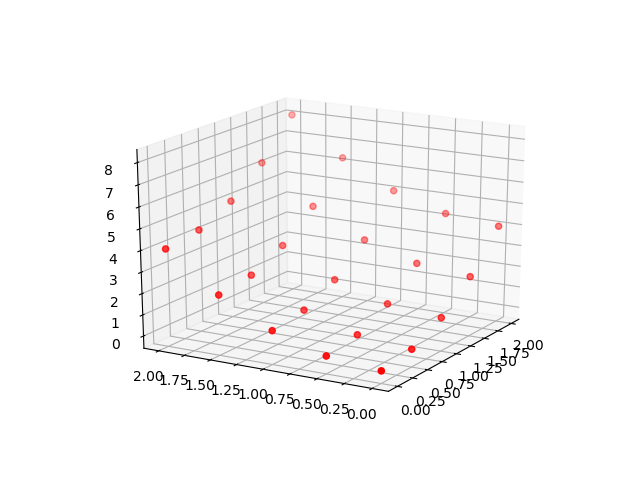
\includegraphics[scale=\myscale,scale=0.5]{figures/pythonxy-numpy1}
  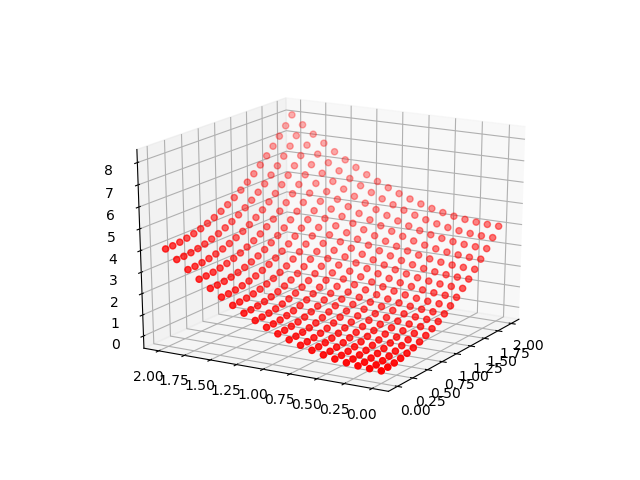
\includegraphics[scale=\myscale,scale=0.5]{figures/pythonxy-numpy2}
  \end{center}


\end{itemize}


%%%%%%%%%%%%%%%%%%%%%%%%%%%%%%%%%%%%%%%%%%%%%%%%%%%%%%%%%%%%%%%%%%%%%
\section{Un peu plus sur numpy}


%--------------------------------------------------------------------
\subsection{Ses propres fonctions}

On peut définir ses propres fonctions.
Dans le cas le plus simple, il n'y a rien de spécial à faire.

\begin{center}
\begin{minipage}{0.9\textwidth}
\begin{lstlisting}    
def ma_formule(x):
	return np.cos(x)**2 - np.sin(x)**2
\end{lstlisting}
\end{minipage}
\end{center}
Alors \ci{ma_formule(X)} renvoie le résultat, que $X$ soit un nombre, un vecteur ou un tableau.

On peut aussi utiliser les fonctions \og{}lambda\fg{} :
\mycenterline{\ci{f = lambda n:n*(n+1)/2}}
à utiliser sous la forme usuelle \ci{Y = f(X)}.


%--------------------------------------------------------------------
\subsection{Ses propres fonctions (suite)}

Par contre, la fonction suivante ne sait traiter directement ni un vecteur ni un tableau, à cause du test de positivité.
\begin{center}
\begin{minipage}{0.9\textwidth}
\begin{lstlisting} 
def valeur_absolue(x):
	if x >= 0:
		return x
	else:
		return -x
\end{lstlisting}
\end{minipage}
\end{center}


Un appel \ci{valeur_absolue(x)} fonctionne lorsque $x$ est un nombre, mais si $X$ est un vecteur ou un tableau alors un appel \ci{valeur_absolue(X)} renvoie une erreur. Il faut \og{}vectoriser\fg{}\index{numpy@\numpy!vectorize@\ci{vectorize()}} la fonction par la commande :
\mycenterline{\ci{vec_valeur_absolue = np.vectorize(valeur_absolue)}}

Maintenant \ci{vec_valeur_absolue(X)} fonctionne pour les nombres, les vecteurs et les tableaux.

\begin{remarque*}
Il peut être utile de préciser que chaque composante de sortie doit être un nombre flottant :

\mycenterline{\ci{vec_fonction = np.vectorize(fonction, otypes=[np.float64])}}
\end{remarque*}


%--------------------------------------------------------------------
\subsection{Le zéro et l'infini}

Le module \numpy{} gère bien les problèmes rencontrés lors des calculs. Prenons l'exemple du vecteur $X$ suivant :
\mycenterline{\ci{[-1  0  1  2  3]}}

\begin{itemize}
  \item La commande \ci{1/X} renvoie le vecteur :
\mycenterline{\ci{[-1.                 inf  1.          0.5         0.33333333]}}
La commande émet un avertissement (mais n'interrompt pas le programme). Comme valeur de $1/0$ elle renvoie \ci{inf} pour l'infini $\infty$.\index{numpy@\numpy!inf@\ci{inf}}

  \item La commande \ci{Y = np.log(X)} donne un vecteur $Y$ :
\mycenterline{\ci{[       nan       -inf 0.         0.69314718 1.09861229]}}
où \og{}\ci{nan}\fg{}\index{numpy@\numpy!nan@\ci{nan}} est une abréviation de \emph{Not A Number} car le logarithme n'est pas défini pour des valeurs négatives et \ci{-inf} représente $-\infty$ (qui est la limite en $0$ du logarithme).

  \item La commande \ci{Z = np.exp(Y)} donne \ci{[nan  0.  1.  2.  3.]}. Ce qui est presque le vecteur $X$ de départ et cohérent avec la formule $\exp(\ln(x))=x$ pour $x>0$.
\end{itemize}

%--------------------------------------------------------------------
\subsection{Utilisation comme une liste}

Soit le vecteur $X$ défini par la commande :
\mycenterline{\ci{X = np.linspace(0,10,num=100)}}

Pour récupérer une partie du vecteur, la syntaxe est la même que pour les listes \Python.

\begin{itemize}
\item \'Elément de rang $50$ : \ci{X[50]}.
\item Dernier élément : \ci{X[-1]}. 
\item \'Eléments de rang $10$ à $19$ : \ci{X[10:20]}.
\item \'Eléments du début au rang $9$ : \ci{X[:10]}.
\item \'Eléments du rang $90$ à la fin : \ci{X[90:]}.
\end{itemize}

\medskip

Voici des fonctionnalités moins utiles.

\begin{itemize}
  \item Ajouter un élément à un vecteur avec \ci{append()}.
  Par exemple si \ci{X = np.arange(0,5,0.5)} alors la commande
  \ci{Y = np.append(X,8.5)} construit un nouveau vecteur qui se termine par l'élément $8.5$.
  
  \item Revenir à une liste. Utiliser la conversion \ci{list(X)} pour obtenir une liste \Python{} à partir d'un vecteur \numpy{}.
  
\end{itemize}



%%%%%%%%%%%%%%%%%%%%%%%%%%%%%%%%%%%%%%%%%%%%%%%%%%%%%%%%%%%%%%%%%%%%%
\section{Matplotlib : deux variables}

%--------------------------------------------------------------------
\subsection{Graphes}

On calcule d'abord une grille $(X,Y)$ de points et les valeurs $Z$ de la fonction sur cette grille. Ensuite le tracé du graphe se fait grâce à l'instruction \ci{plot_surface(X, Y, Z)}.\index{matplotlib@\matplotlib!plot-surface@\ci{plot_surface()}}


\begin{minipage}{0.53\textwidth}
\begin{lstlisting}   
import numpy as np
import matplotlib.pyplot as plt
from mpl_toolkits.mplot3d import Axes3D

n = 5
VX = np.linspace(-2.0, 2.0, n)
VY = np.linspace(-2.0, 2.0, n)
X,Y = np.meshgrid(VX, VY)

def f(x,y):
	return x**2-y**2

Z = f(X,Y)

fig = plt.figure()
ax = plt.axes(projection='3d')
ax.view_init(40, -30)

ax.plot_surface(X, Y, Z)
 
plt.show()

\end{lstlisting}
\end{minipage}
\begin{minipage}{0.45\textwidth}
\begin{center}
  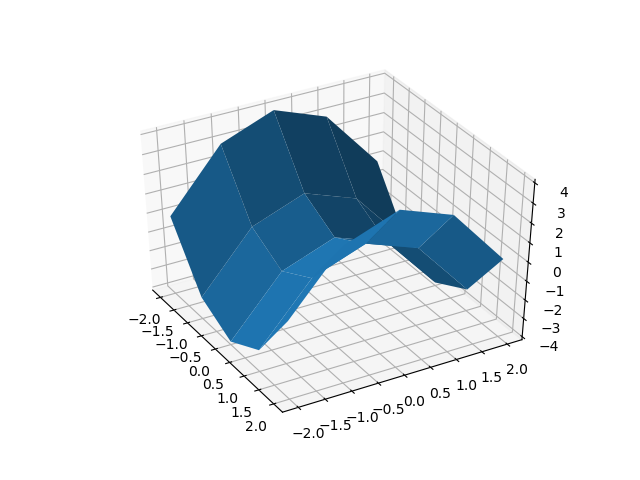
\includegraphics[scale=\myscale,scale=0.45]{figures/pythonxy-selle-1}

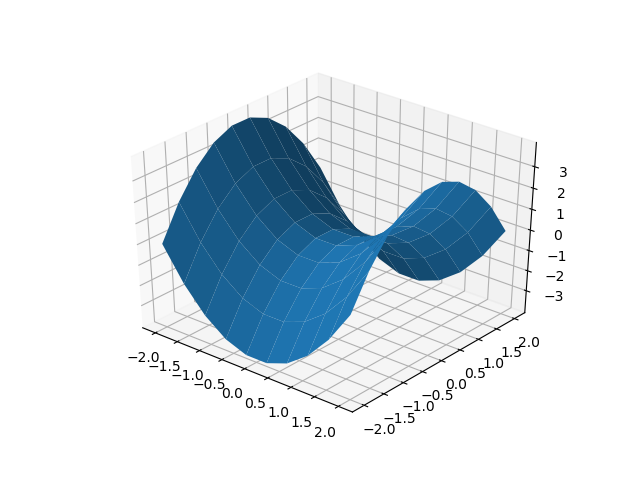
\includegraphics[scale=\myscale,scale=0.45]{figures/pythonxy-selle-2}

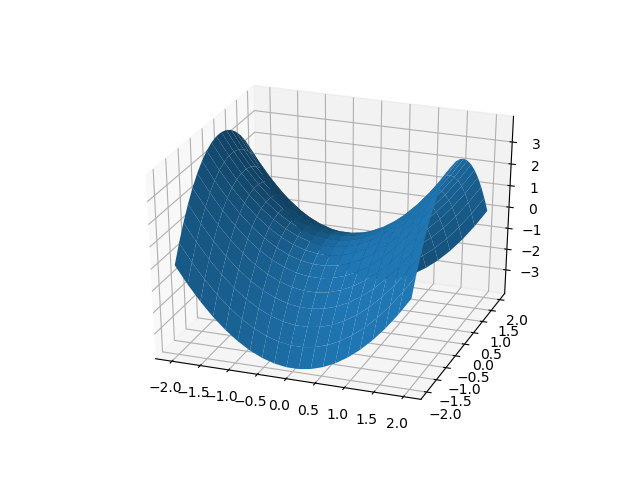
\includegraphics[scale=\myscale,scale=0.45]{figures/pythonxy-selle-3}
\end{center}
\end{minipage}

Si on augmente $n$, la grille est plus dense et la surface dessinée   paraît plus lisse car il y a davantage de polygones. Les tracés de la \og{}selle de cheval\fg{} ci-dessus sont effectués pour $n=5$, $n=10$, puis $n=20$. L'affichage 3D permet de tourner la surface pour mieux l'appréhender. On peut aussi fixer le point de vue avec \ci{view_init()}.

Il existe de multiples variantes et coloriages possibles.

\begin{minipage}{0.45\textwidth}
\begin{center}
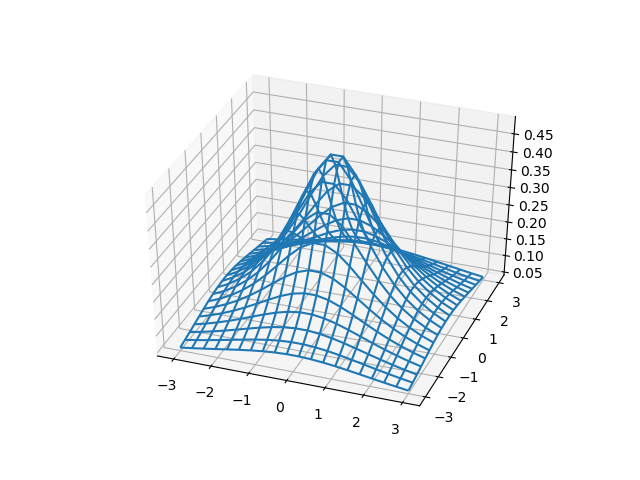
\includegraphics[scale=\myscale,scale=0.6]{figures/pythonxy-surface-1}
\end{center}
\end{minipage}
\begin{minipage}{0.45\textwidth}
\begin{center}
$$f(x,y) = \frac{1}{2+x^2+y^2}$$

\ci{plot_wireframe(X, Y, Z)}
\end{center}
\end{minipage}


\begin{minipage}{0.45\textwidth}
\begin{center}
$$f(x,y) = |x|+|y|$$

Barre des couleurs
\end{center}
\end{minipage}
\begin{minipage}{0.45\textwidth}
\begin{center}
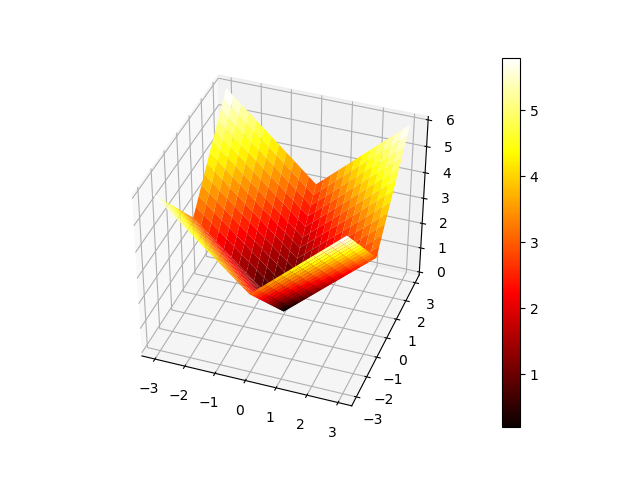
\includegraphics[scale=\myscale,scale=0.6]{figures/pythonxy-surface-2}
\end{center}
\end{minipage}


\begin{minipage}{0.45\textwidth}
\begin{center}
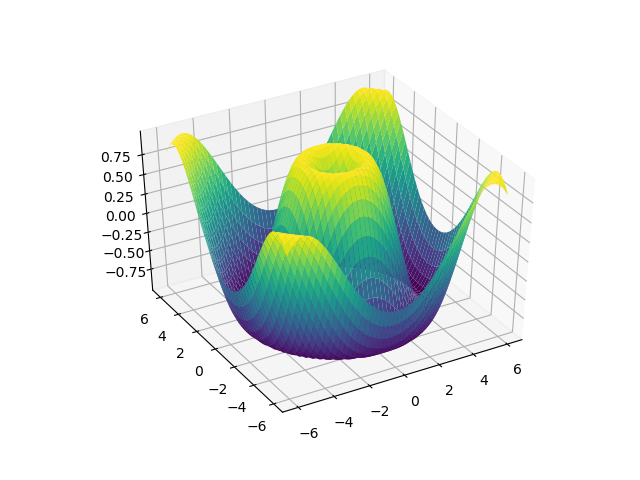
\includegraphics[scale=\myscale,scale=0.6]{figures/pythonxy-surface-3}
\end{center}
\end{minipage}
\begin{minipage}{0.45\textwidth}
\begin{center}
$$f(x,y) = \sin\left(\sqrt{x^2+y^2}\right)$$
\end{center}
\end{minipage}



%--------------------------------------------------------------------
\subsection{Lignes de niveau}

Il nous sera particulièrement utile de trouver les lignes de niveau d'une fonction $f$, en particulier pour trouver tous les $(x,y)$ tels que $f(x,y)\ge0$ par exemple.
Le principe est similaire au tracé de la surface et s'effectue par la commande : 
\mycenterline{\ci{plt.contour(X, Y, Z)}}
\index{matplotlib@\matplotlib!contour@\ci{contour()}}
\begin{center}
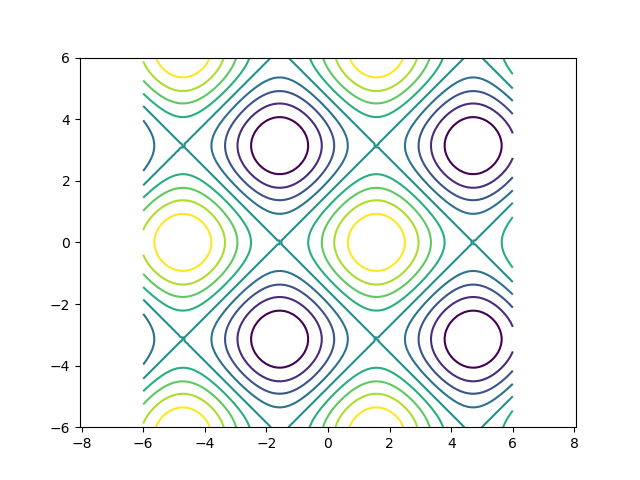
\includegraphics[scale=\myscale,scale=0.8]{figures/pythonxy-niveau-2d-1}
\end{center}

\begin{minipage}{0.45\textwidth}
On peut préciser le nombre de niveaux tracés
\ci{plt.contour(X, Y, Z, nb_niveaux)} (ci-dessus). Le graphe en dimension $3$ ci-contre.
\end{minipage}
\begin{minipage}{0.45\textwidth}
\begin{center}
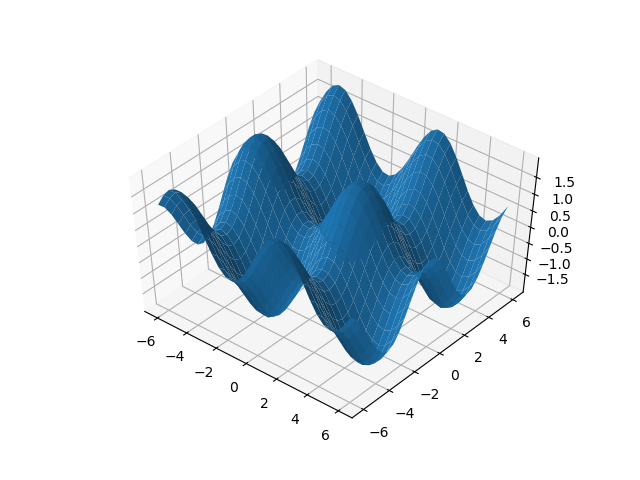
\includegraphics[scale=\myscale,scale=0.5]{figures/pythonxy-niveau-3d-1}
\end{center}
\end{minipage}


\begin{center}
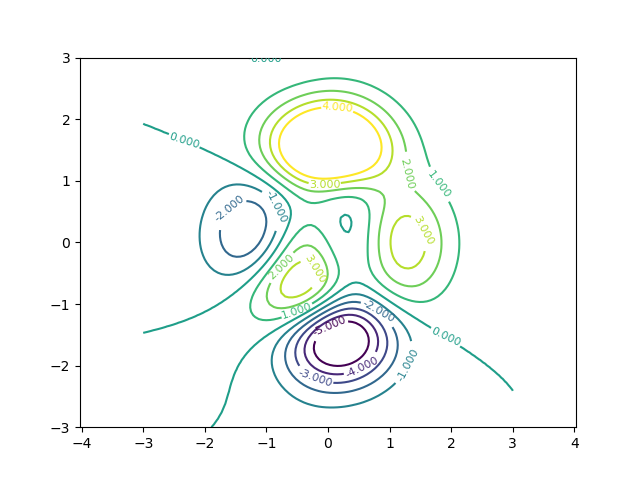
\includegraphics[scale=\myscale,scale=0.8]{figures/pythonxy-niveau-2d-2}
\end{center}


\begin{minipage}{0.5\textwidth}
\begin{center}
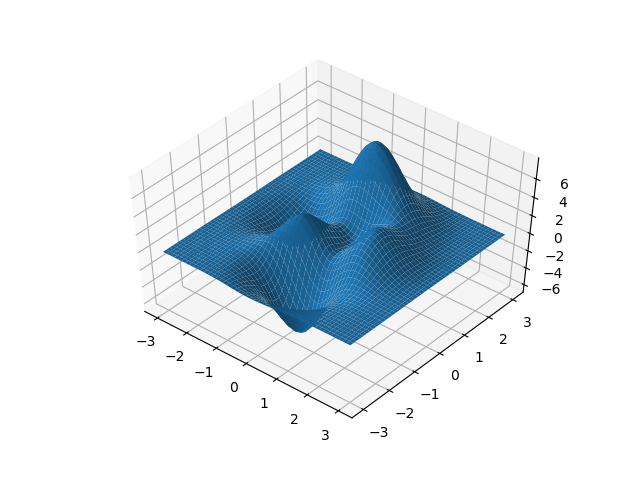
\includegraphics[scale=\myscale,scale=0.5]{figures/pythonxy-niveau-3d-2}
\end{center}
\end{minipage}
\begin{minipage}{0.45\textwidth}
 On peut spécifier les niveaux à afficher par 
  \ci{plt.contour(X, Y, Z, mes_niveaux)} où 
  \ci{mes_niveaux = np.arange(-5,5,1)} par exemple.
  On peut en profiter pour afficher la valeur du niveau, comme l'altitude sur une carte topographique (ci-dessus les lignes de niveau, ci-contre le graphe 3D).
\end{minipage}



\begin{center}
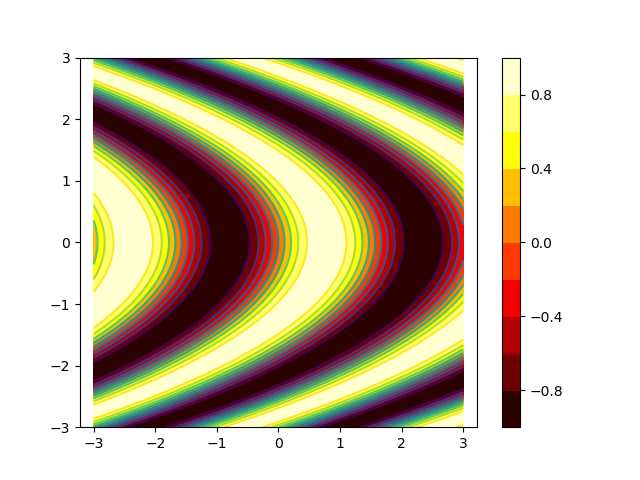
\includegraphics[scale=\myscale,scale=0.8]{figures/pythonxy-niveau-2d-3}
\end{center}

\begin{minipage}{0.45\textwidth}
\ci{plt.contourf(X, Y, Z)} colorie le plan au lieu de tracer les lignes de niveau (ci-dessus les lignes de niveau, ci-contre le graphe 3D).
\end{minipage}
\begin{minipage}{0.45\textwidth}
\begin{center}
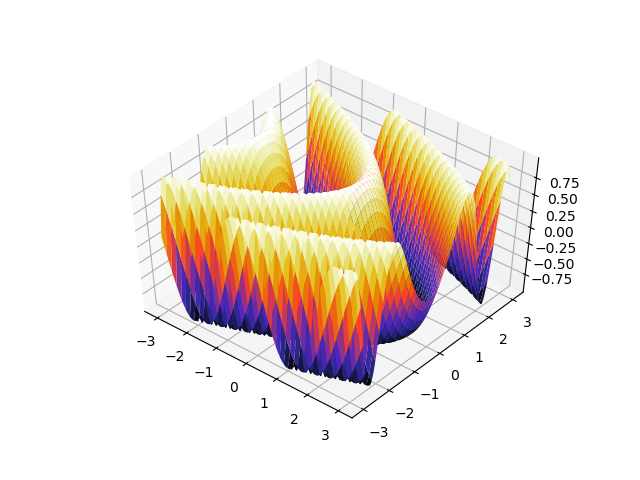
\includegraphics[scale=\myscale,scale=0.5]{figures/pythonxy-niveau-3d-3}
\end{center}
\end{minipage}



On peut même tracer les lignes de niveau sous la surface comme ci-dessous.
\begin{center}
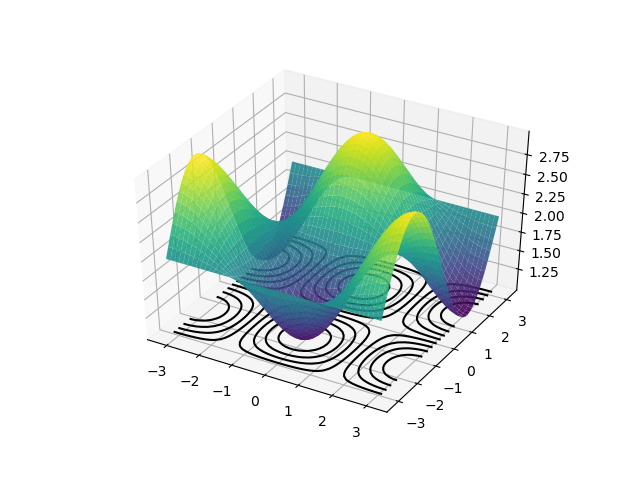
\includegraphics[scale=\myscale,scale=0.9]{figures/pythonxy-niveau-3d-4}
\end{center}

\end{document}
